\documentclass{article}

\usepackage{graphicx}
\usepackage{tikz}
\usepackage{tikzsymbols}
\usetikzlibrary{calc,patterns,shapes.geometric}
\pagestyle{empty}
\usepackage[margin=0pt]{geometry}
\geometry{papersize={14in,12in}}

\def\centerarc[#1](#2)(#3:#4:#5){\draw[#1] ($(#2)+({#5*cos(#3)},{#5*sin(#3)})$) arc (#3:#4:#5);}

\begin{document}
	\begin{figure}
		\centering
		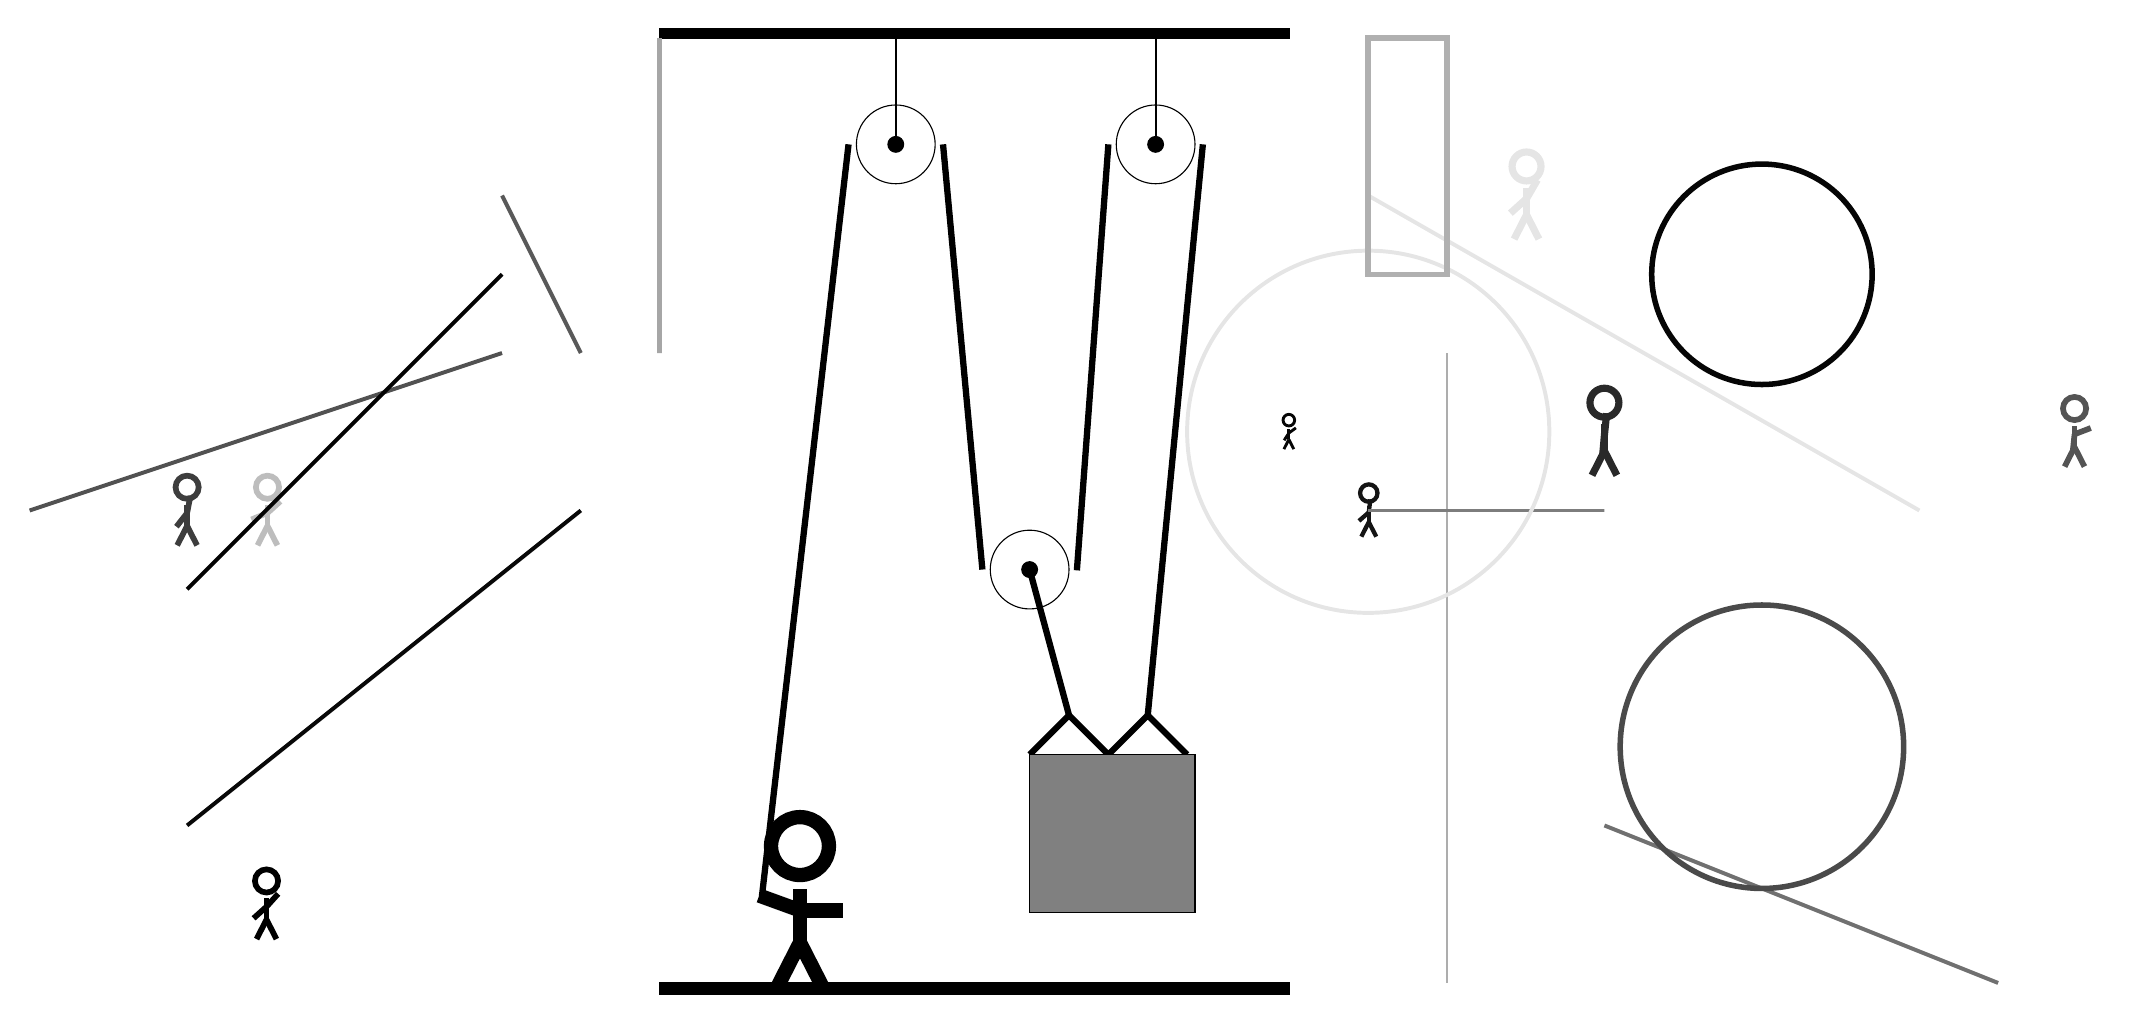
\begin{tikzpicture}
			%%%%% START %%%%%
			
			\draw[fill=black] (-2, 9) rectangle (6, 9.125);
			
			\node[line width=0.5mm, color=black!10] at (9, 7) {\Strichmaxerl[5][42][60]};
			
			\draw[line width=0.5mm, color=black!65](-4, 7) -- (-3, 5);
			\node[line width=0.4mm, color=black!67] at (16, 4) {\Strichmaxerl[4][84][21]};
			\node[line width=0.6mm, color=black!26] at (-7, 3) {\Strichmaxerl[4][22][42]};
			\node[line width=0.4mm, color=black!76] at (-8, 3) {\Strichmaxerl[4][52][79]};
			\node[line width=0.3mm, color=black!100] at (-7, -2) {\Strichmaxerl[4][42][48]};
			
			\draw[line width=0.5mm, color=black!56](10, -1) -- (15, -3);
			\node[line width=0.5mm, color=black!92] at (7, 3) {\Strichmaxerl[3][41][83]};
			\node[line width=0.4mm, color=black!98] at (6, 4) {\Strichmaxerl[2][57][36]};
			\draw[line width=0.2mm, color=black!32] (8, -3) rectangle (8, 5);
			\draw[line width=0.6mm, color=black!35] (-2, 9) rectangle (-2, 5);
			\draw[line width=0.4mm, color=black!51] (7, 3) rectangle (10, 3);
			\draw [line width=0.7mm, color=black!71](12, 0) circle (1.8);
			
			\node[line width=0.2mm, color=black!84] at (10, 4) {\Strichmaxerl[5][85][84]};
			\draw[line width=0.5mm, color=black!97](-3, 3) -- (-8, -1);
			\draw [line width=0.5mm, color=black!10](7, 4) circle (2.3);
			
			\draw[line width=0.5mm, color=black!10](7, 7) -- (14, 3);
			\draw[line width=0.5mm, color=black!68](-4, 5) -- (-10, 3);
			\draw[line width=0.7mm, color=black!31] (7, 6) rectangle (8, 9);
			
			\draw[line width=0.5mm, color=black!99](-4, 6) -- (-8, 2);
			\draw [line width=0.7mm, color=black!98](12, 6) circle (1.4);
			
			\draw (1, 7.65) circle (0.5);
			\draw[fill=black] (1, 7.65) circle (0.1);
			\draw[thick] (1, 7.65) -- (1, 9);
			
			\draw (4.3, 7.65) circle (0.5);
			\draw[fill=black] (4.3, 7.65) circle (0.1);
			\draw[thick] (4.3, 7.65) -- (4.3, 9);
			
			\draw (2.7, 2.25) circle (0.5);
			\draw[fill=black] (2.7, 2.25) circle (0.1);
			
			\draw[line width=0.8mm]  (2.7, -0.1) -- (3.2, 0.4) -- (3.7, -0.1) -- (4.2, 0.4) -- (4.7, -0.1);
			\draw[fill=black!50] (2.7, -0.1) rectangle (4.8, -2.1);
			
			\draw[line width=0.8mm](-0.7, -1.9) -- (0.4, 7.65);
			\centerarc[line width=0.8mm](1, 7.65)(0:180:0.6);
			\draw[line width=0.8mm](1.6, 7.65) -- (2.1, 2.25);
			\centerarc[line width=0.8mm](2.7, 2.25)(180:370:0.6);
			\draw[line width=0.8mm] (3.3, 2.24) -- (3.7, 7.65);
			\centerarc[line width=0.8mm](4.3, 7.65)(0:180:0.6);
			\draw[line width=0.8mm](4.2, 0.4) -- (4.9, 7.65);
			\draw[line width=0.8mm] (3.2, 0.4) -- (2.7, 2.25);
			
			\node at (-0.2, -2) {\Strichmaxerl[10][-20][0]};
			
			\draw[fill=black] (-2, -3) rectangle (6, -3.15);
			
			%%%%% END %%%%%
		\end{tikzpicture}
	\end{figure}	
\end{document}